\subsection{Methodological Literature}

Based on the systematic review and its coding, the first data set we
assess is a database of scale validations. We bring together the scales
suggested in previous reviews as well as validation studies we
identified in our own review. Throughout our literature review we found
five major works that reviewed the measurement of acculturation
\citep{Celenk2011, Maestas2000, Matsudaira2006, Wallace2010, Zane2004}.
After removal of duplicate scales, we added any scale validation that
was present in our own systematic review but not included in the
previous reviews. For each measure we extracted the full item list as
well as the item scoring prior to coding. A comprehensive and
interactive database of the scales, with reference- and publication
information, as well as our experience elements and -context coding is
available in our online supplementary information as well as on our open
science repository (\hl{OSF and/or github citation here}).

\subsubsection{Methods}

Taken together these five reviews collected a total of 97 scales. From
our own review we added 151 additional validation studies. After
removing duplicates this meant that we considered a total of 247 unique
scales for our coding. Of these scales we ultimately had to exclude 23,
because they were either not accessible or did not fit the the topic of
our review (see Table \ref{tab:ScalesExclusion}). About a quarter of
scales (24.29\%) included majority group members in their validation
studies. The earliest included validation was from 1948 with a majority
of scales being validated around the turn of the 21\textsuperscript{st}
century and the most recent included validation study was published in
2020.

\begin{table}

\caption{(\#tab:ScalesExclusion)Reasons for Exclusion}
\begin{tabular}[t]{lc}
\toprule
Exclusion Reason & Frequency\\
\midrule
not migration & 14\\
items not included & 8\\
search pending & 5\\
not accessible & 4\\
not found & 3\\
not acculturation & 2\\
majority focussed & 1\\
not found probably the same as Tsai et al. 2000 & 1\\
only language (no scale) & 1\\
same as S-029 & 1\\
uses other scale & 1\\
\bottomrule
\end{tabular}
\end{table}


\subsubsection{Results}

With our main aim of examining the experience structure within the
scales, we examined whether scales included a specific experience
elements but also examined the used elements in their complex
combinations. In terms of general inclusion of elements, most studies
included a measure of cognition (86.43\%) and behavior (75.57\%),
whereas only roughly half the studies included a measure of affect
(52.49\%) and only a fourth of the scales included a measure of desires
(23.98\%). However, only a minority of scales included only a single
aspect. There were only 14 scales that exclusively relied on cognitions
(6.33\%) and 20 scales that measured only behaviors (9.05\%). Yet,
inversely, there were also only 30 scales that measured all four aspects
(13.57\%). Most studies measured two (41.63\%) or three (28.05\%)
aspects. A majority of scales either measured behavioral and cognitive
aspects (25.79\%) or behavioral, cognitive, and affective elements
(21.27\%; also see Figure \ref{fig:ElementsScales} and Table
\ref{tab:ScaleElementCooccurrences}). Looking at the number of aspects
measured together we also see substantial differences in what kind of
scales include a certain aspect. Scales that included cognitions
measured an average of 2.56 aspects, scales measuring behavior, on
average, measured a 2.57, while scales that included affect measures had
a complexity average of 2.97 and scales measuring desires even measured
an average of 3.42 aspects per scale. Thus, most scales measure multiple
dimensions, yet they focus on external accessible aspects of
psychological acculturation (i.e., behavior and cognition), less of what
is considered `internal' or `subjective' (i.e., affect and desires).
This is further underscored by the observation that there were only 3
scales that exclusively measured emotional acculturation and not a
single scale that exclusively focused on motivational acculturation
(while this was the case for both cognitions and behaviors). And if
emotional or desire aspects were measured they were on average measured
in scales that had already included more experience aspects.

\begin{figure}[h]
\centering
\caption{Scales: Bar graph of the experience element combinations.}
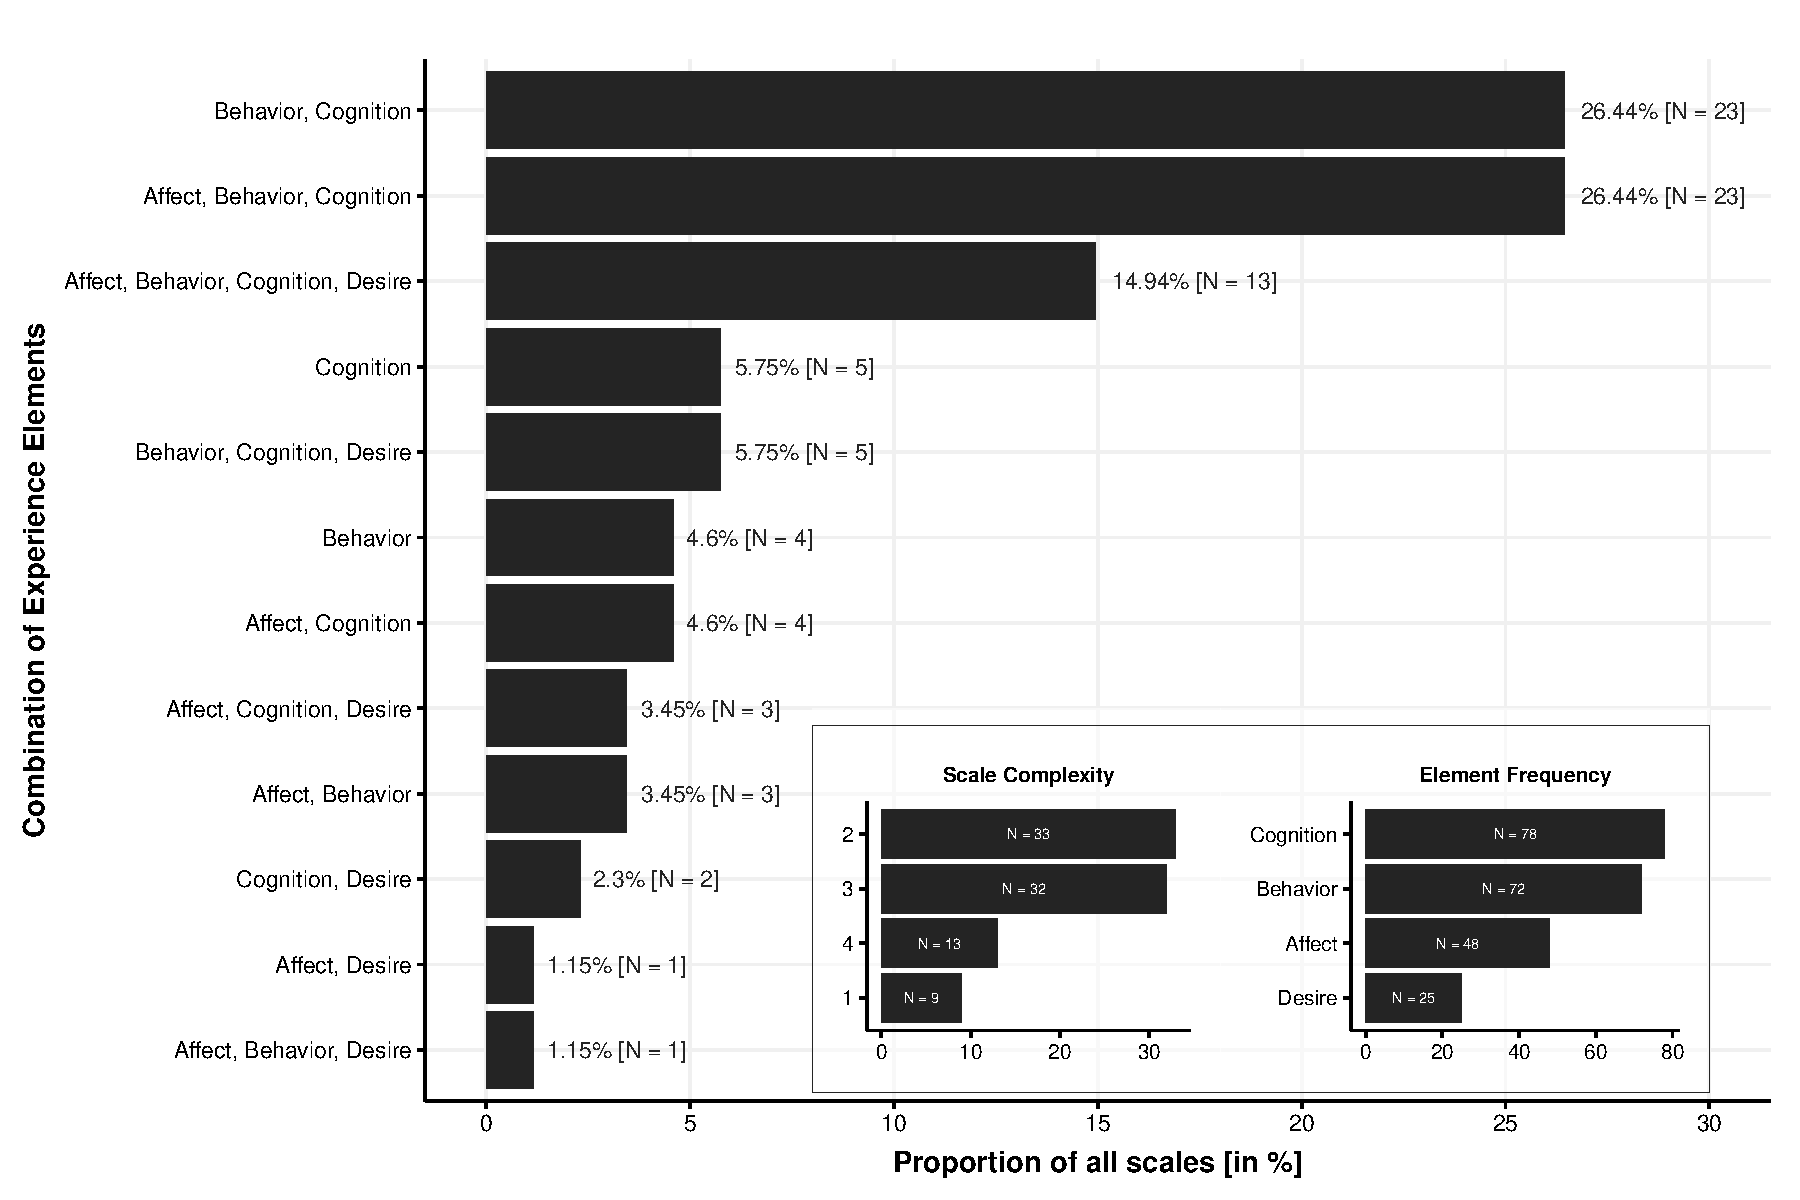
\includegraphics[width=\textwidth]{Figures/ABCDFreq-1}
\label{fig:ElementsScales}
\end{figure}

\begin{table}

\caption{\label{tab:ScaleElementCooccurrences}Scales: Element Co-occurrence Matrix}
\begin{tabular}[t]{lcccc}
\toprule
  & Affect & Behavior & Cognition & Desire\\
\midrule
Affect & 48 & 40 & 43 & 18\\
Behavior & 40 & 72 & 64 & 19\\
Cognition & 43 & 64 & 78 & 23\\
Desire & 18 & 19 & 23 & 25\\
\bottomrule
\end{tabular}
\end{table}

To assess the process focus of the scales we also assessed the migration
time the scale validators considered. Except for a single scale that was
validated for potential migrants, all scales were validated using
cross-sectional data after the migrant arrived in the settlement
society. This is in line with observations by previous reviews of the
field \citep[e.g.,][]{Brown2011}.

\subsection{Empirical Literature}

After analysis of the scales validations, we assessed the broader
empirical works we collected within the systematic review. We first
looked at all available empirical publications (incl.~books, chapters,
and dissertations). We later also assessed differences between journal
fields to assess differences between fields.

\subsubsection{Methods}

The search produced a total of 1629 results to which we added 399
articles through contacts with experts in the field and from referenced
works within the review. We subsequently screened out results that did
not fit into our review. After duplicate removal (\(N_{excluded}\) =
300, \(N_{screened}\) = 1329), we excluded 383 results in the title
screening as well as an additional 272 results during the abstract
screening. Of the remaining 674 results, 666 papers presented empirical
work on acculturation and were coded. The 8 non-empirical results were
reviews, which were not coded because they did not measure cultural
adaptation. During the full text coding we excluded an additional 140
results because they were either not relevant or were not accessible
(for exclusion reasons see Table \ref{tab:EmpiricalExclusion} and for
our PRISMA diagram see Figure \ref{fig:PRISMA}).

\begin{figure}[h]
\centering
\caption{PRISMA diagram. Position still undecided. Currently generated in R based on n(row) maybe make prettier.}
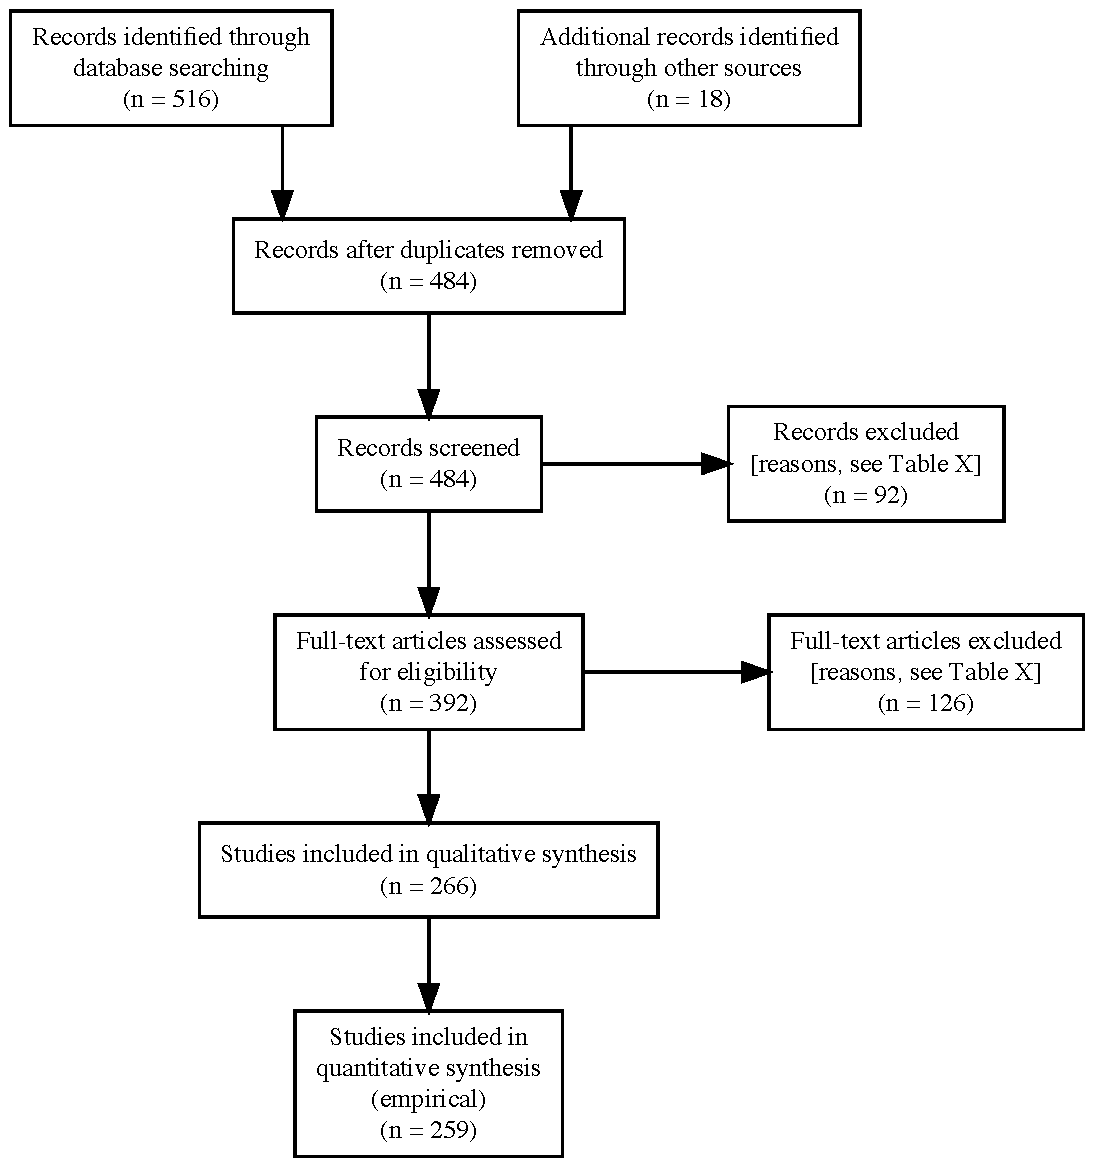
\includegraphics[width=\textwidth]{Figures/PRISMA}
\label{fig:PRISMA}
\end{figure}

\begin{table}

\caption{\label{tab:EmpiricalExclusion}Exclusion Reasons Empirical Literature}
\centering
\begin{tabular}[t]{lccc}
\toprule
\multicolumn{1}{c}{ } & \multicolumn{3}{c}{Screening} \\
\cmidrule(l{3pt}r{3pt}){2-4}
Exclusion Reason & Title & Abstract & Full Text\\
\midrule
not migration & 36 & 27 & \\
not acculturation & 19 & 49 & \\
not experience & 19 & 24 & \\
not migrant & 17 & 18 & \\
not measured &  & 8 & 2\\
re-migration &  & 1 & \\
thesis not accessible &  &  & 13\\
book not accessible &  &  & 4\\
items not accessible &  &  & 4\\
article not accessible &  &  & 2\\
should still be coded &  &  & 1\\
\bottomrule
\end{tabular}
\end{table}


Of the final works we coded, 452 were journal articles, 68 theses, and 6
book chapters. Most studies presented quantitative data (\textit{N} =
464), mixed methods (\textit{N} = 39), or qualitative data (\textit{N} =
20), while the remaining 3 manuscripts were reviews of empirical data.
Notably, a majority of the empirical investigations did not share common
measures of cultural adaptation -- 390 studies used measures that were
reported a maximum of five times, with a considerable majority of papers
using new or ad-hoc measures of cultural adaptation. Less than a fifth
of studies included the local majority in the study (\textit{N} = 77,
14.69\%). Cultural adaptation most frequently was a predictor variable
(\textit{N} = 285, 54.39\%), a dependent variable (\textit{N} = 148,
28.24\%), or a correlation variable (\textit{N} = 37, 7.06\%) in the
empirical works. This pattern was mirrored when looking at the focus of
the papers, where a majority of the papers had acculturation as their
main focus (\textit{N} = 153, 29.48\%), with other bodies of work
focusing on health outcomes (\textit{N} = 51, 9.83\%), or inter-group
relations (\textit{N} = 18, 3.47\%) as their main outcomes. The earliest
included study was published in 1948, with a strong increase of
publications after the year 2000, and a peak of publications in 2012. We
provide full descriptions of descriptive data extractions and additional
information about the data description in Online Supplementary
Information \hl{X}.

\paragraph{Field of Publication}

For the broader empirical literature, we also collected additional data
on the field the studies were published in. To assess the differences
between fields we merged the `Scimago Journal Ranking Database'
\citep{SCImago2020} with our data base. For all available journal
articles we added information on key journal metrics (incl.~H index,
impact factor, and data on the field and audiences). This also meant
that dissertations, book chapters, and books were excluded from this
analysis because data on their publishers is not readily available or
unreliable. Additionally, 10 journals were not included in the Scimago
database (likely because they do not have an ISSN identifier or were
discontinued before 1996, see Online Appendix \hl{X}, Table \hl{X} for
the missing journals). We ultimately had journal metrics for 437
empirical articles.

To summarize the journal data we then classified the journal fields into
super-ordinate discipline codes. These discipline codes are based in
part on U.S. Department of Education's subject classifications
\citep[i.e., CIP;][]{InstituteofEducationSciences2020}, the U.K.
academic coding system
\citep[JACS 3.0;][]{HigherEducationStatisticsAgency2013}, the Australian
and New Zealand Standard Research Classification
\citep[ANZSRC 2020;][]{AustralianBureauofStatistics2020}, as well as the
Fields of Knowledge project \citep{ThingsmadeThinkable2014}. We
ultimately classified each journal into one of four mutually exclusive
disciplines (psychology: \textit{N} = 131, multidisciplinary: \textit{N}
= 103, Medicine, Nursing, and Health: \textit{N} = 146, and Social
Sciences (miscellaneous): \textit{N} = 45. For a full discussion of the
classifications see Online Supplementary Materials \hl{X}).

\subsubsection{Results}

We assessed the role of experience aspects in the measurement and then
compared differences between fields.

\paragraph{General}

In terms of the overall frequencies of experience elements, the broader
empirical data mirrored that of the validation studies. Most studies
included a measure of cognition (80.04\%) and behavior (82.13\%),
whereas only about half of all studies included a measure of affect
(49.05\%) and less than a fifth of the studies included a measure of
desires (17.11\%). Yet, only 119 studies focused on a single experience
aspect (\(N_{behavior\ only}\) = 75, \(N_{cognition\ only}\) = 38,
\(N_{emotion\ only}\) = 6). Similarly, only 42 papers included measures
of all four experience aspects (7.98\%). Most studies measured three
(34.98\%) or two aspects (34.41\%). Different from the scale
validations, within the broader empirical works, most works included
measures of emotions, behaviors, and cognitions (\textit{N} = 153,
29.09\%), with a further substantial number of articles measuring
behaviors and cognitions (\textit{N} = 120, 22.81\%. Also see Figure
\ref{fig:EmpPlotFreq-1} and Table
\ref{tab:EmpiricalElementCooccurrences}). Looking at the number of
aspects measured together we again see substantial differences in what
kind of scales include the individual aspects. Scales that included
cognitions measured an average of 2.54 aspects, scales measuring
behavior, on average, measured 2.43, while scales that included affect
measured an average of 2.93 experience aspects and scales measuring
desires even measured an average of 3.28 experience aspects. Thus, not a
single study measured only motivation (i.e., desires), and measures of
desires remained mostly limited to scales that were already measuring
many of the other experience aspects. The results exacerbate the pattern
found in the scale validations, complex measures and conceptions of
acculturation are seen infrequently and exteral aspects of cognition and
behavior remain the focus of most studies.

\begin{figure}[h]
\centering
\caption{Empirical Literature: Bar graph of the experience element combinations.}
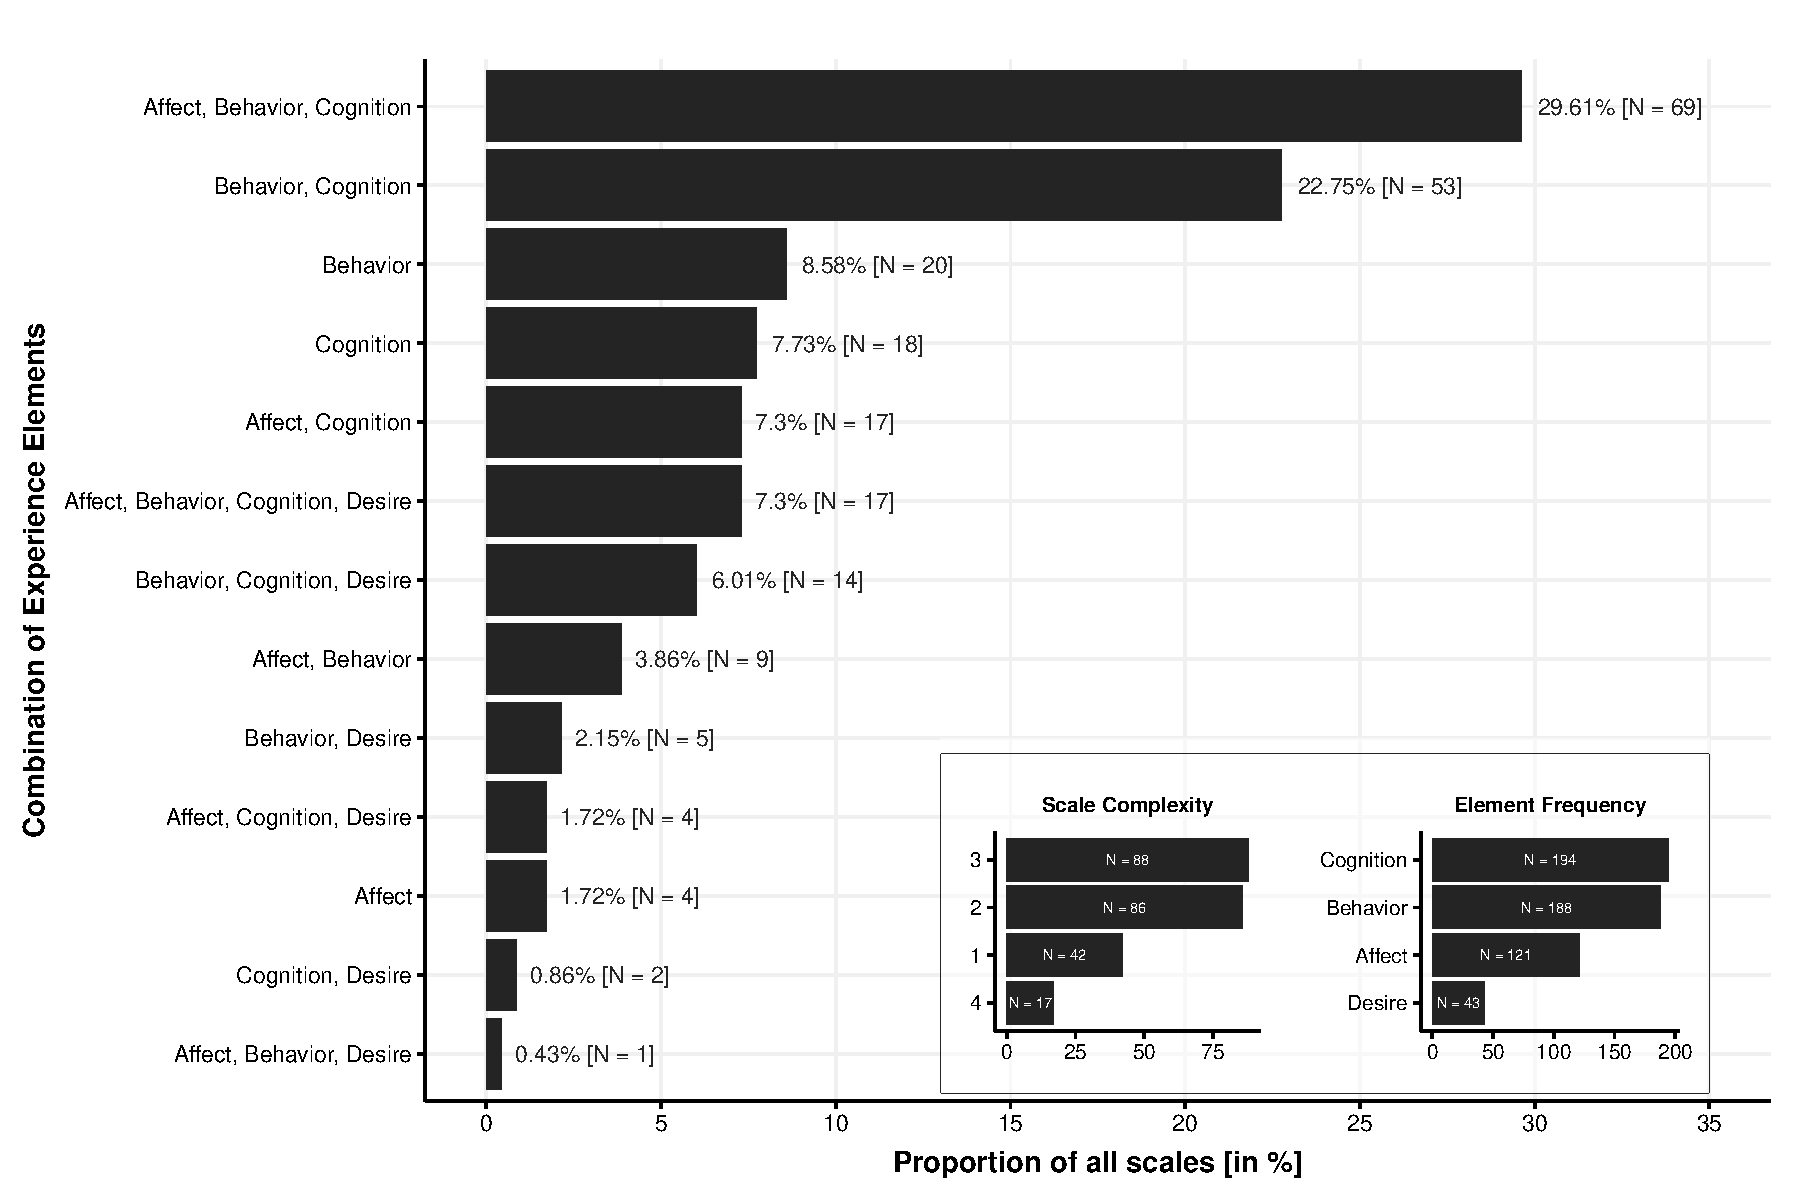
\includegraphics[width=\textwidth]{Figures/EmpPlotFreq-1}
\label{fig:EmpPlotFreq-1}
\end{figure}

\begin{table}

\caption{\label{tab:EmpiricalElementCooccurrences}Empirical Literature: Element Co-occurrence Matrix}
\centering
\begin{tabular}[t]{lcccc}
\toprule
  & Affect & Behavior & Cognition & Desire\\
\midrule
Affect & 121 & 96 & 107 & 22\\
Behavior & 96 & 188 & 153 & 37\\
Cognition & 107 & 153 & 194 & 37\\
Desire & 22 & 37 & 37 & 43\\
\bottomrule
\end{tabular}
\end{table}


To assess the process focus of the broader empirical works, we again
assessed when in the migration process the data was collected and we
additionally assessed the type analysis done by the authors. We found
that 512 studies (97.71\%) collected data after the arrival of the
migrant in the new society. Two studies targeted potential migrants and
10 studies collected data prior and following the migration event.
Moreover, only 25 studies included longitudinal data analyses of
psychological acculturation (4.79\%). This observation, again
underscores the arguments that the acculturation literature has thus far
failed to provide data that meaningfully captures migration as a process
\citep[e.g.,][]{Brown2011, Ward2019}.

\paragraph{Fields}

To further assess the comparative utility of the experience framework,
we further assessed differences of experience aspects between academic
fields. We provide more elaborate descriptions of the differences in the
methods, and publication types as well as contextual differences in
terms of sampling procedures, situational domains, analyses, and
cultural contexts in Supplementary Online Material \hl{X}.

We first assessed the references to affect, behavior, cognition, and
desires separately, for each of the disciplines. We find that for all
fields desires (11.64-25.95\% of all measures in the field) and emotions
(37.67-58.78\%) are the least frequently measured elements and medical
journals measure them the least frequently (in proportional terms).
Looking at the common cognitive and behavioral elements the proportions
diverge between the fields. While the multidisciplinary field measured
behaviors (79.61\%) and cognition (79.61\%) almost equally often, in the
medical and general social science journals behaviors were measured
considerably more often than cognitions (\(Behavior_{SoSci}\) = 88.89\%
\textgreater{} \(Cognition_{SoSci}\) = 62.22\%; \(Behavior_{Med}\) =
88.36\% \textgreater{} \(Cognition_{Med}\) = 68.49\%). Inversely, in the
psychological journals cognitions (89.31\%) were measured more often
than behaviors (73.28\%; also see Figure \ref{fig:FieldPlotFreq} B and
A).

When looking at differences in how many different experience aspects
were measured together and patterns within these aspect-combinations,
differences between the fields become increasingly evident (also see
Figure \ref{fig:FieldPlotFreq} A and C). While `affect, behavior, and
cognition' and `behavior, and cognition' measures are common
combinations across all fields, there is less experience complexity and
variation for medical and social science fields. There were
statistically significant mean differences between the fields in terms
of how many experience aspects were considered (parametric:
\textit{F}(3, 421) = 5.98, \textit{p} = 0.001, non-parametric:
\textit{Kruskal-Wallis} \(\chi^{2}\) = 18.08, \textit{df} = 3,
\textit{p} = 0, \(\eta_{p}^{2}\) = 0.04, 95\%CI{[}0.01, 0.08{]}).
Looking at the mean differences in more detail, empirical works
published in psychological journals had significantly higher average
aspect counts (\textit{M} = 2.47, \textit{SD} = 0.76) than the medical
(\textit{M} = 2.06, \textit{SD} = 0.84) and the general social science
journals (\textit{M} = 2.02, \textit{SD} = 0.75; also see Figure
\ref{fig:FieldPlotComplexityAverage}).

\begin{figure}[h]
\centering
\caption{Scale Complexity and their proportional occurences per field.}
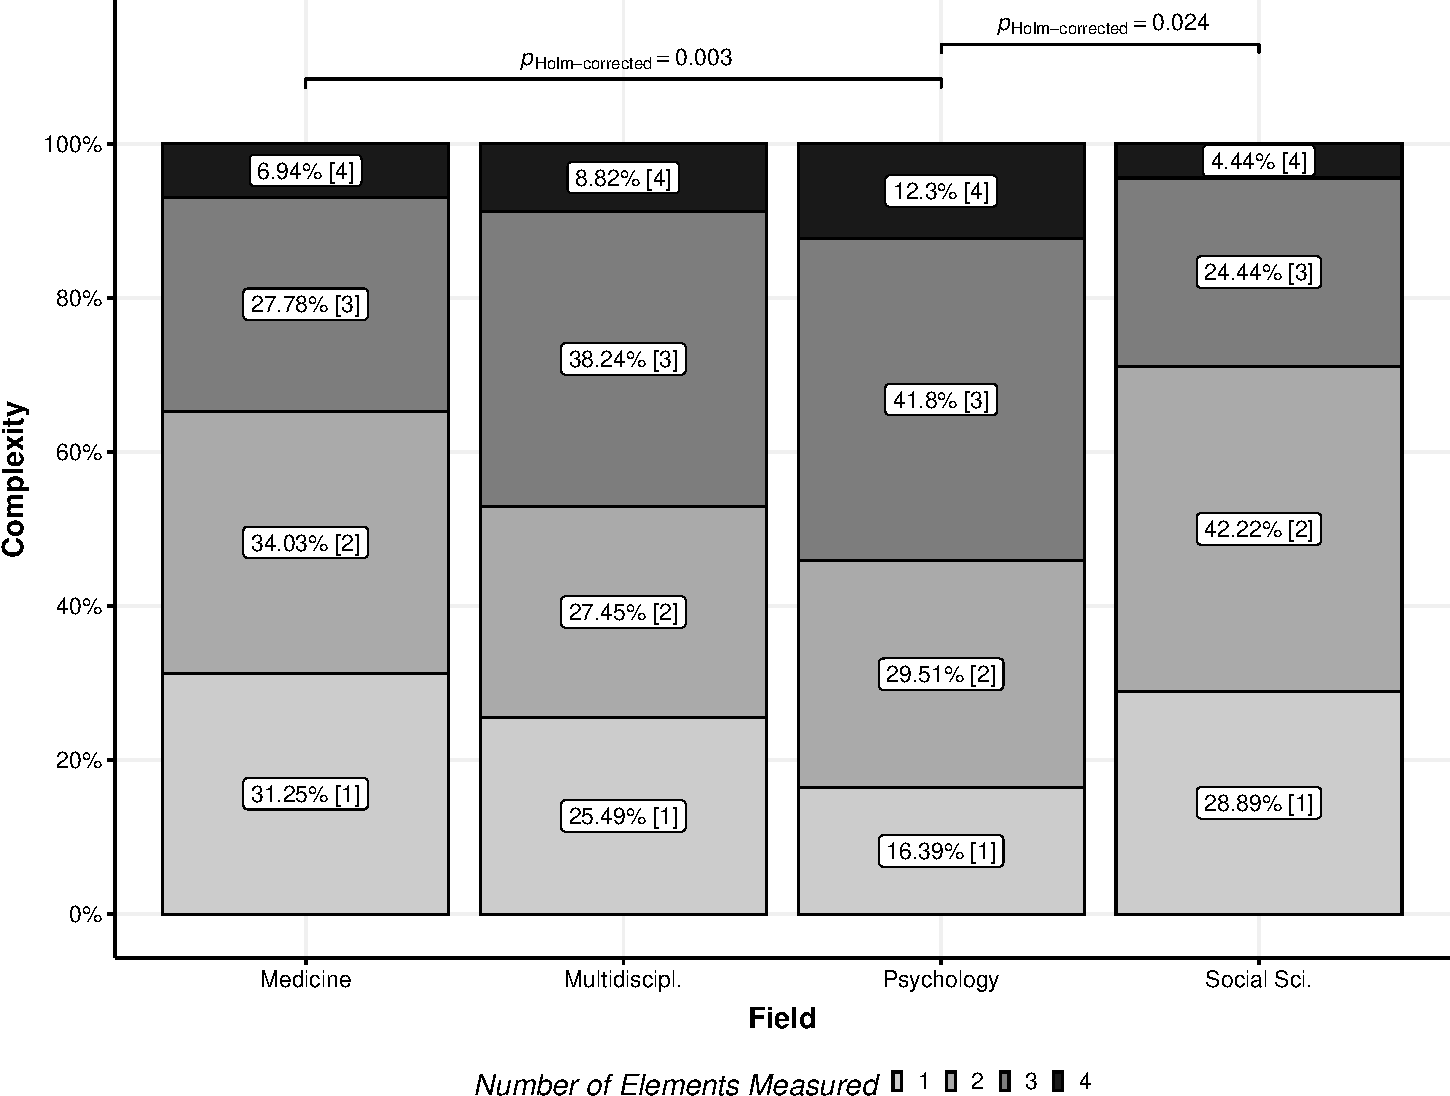
\includegraphics[width=\textwidth]{Figures/FieldPlotComplexityAverage-1}
\label{fig:FieldPlotComplexityAverage}
\end{figure}

Further looking at the qualitative differences of aspect combinations
can be informative as well. For example, there were a mere 3 study
published in a psychological journal that conceptualized cultural
adaptation by behavior alone --- eventhough this is the most common or
second most common conceptualization in the other three fields (also see
Figure \ref{fig:FieldPlotFreq} A). There are also interesting pattern
when one considers how many other elements an aspect is measured with,
within each of the fields. For example, while for all fields motivations
are found in the most complex scales
\footnote{Except for the broader social science journals that do not have many papers measuring motivation in the first place.},
medical and multidisciplinary journals have a substantially higher
average scale complexity when measuring motivations. Inversely,
psychological journal on average report behavioral measures of cultural
adaptation in more complex scales. This hints to a pattern, where
complexity might indicate relative importance of an aspect within the
field -- where only scales that already have a broad and diverse measure
also include the aspects that are usually measured less within a field
(also see Figure \ref{fig:FieldElementComp}). We did not test these
differences formally because the number of experience aspects were not
independent between scales. There are likely other and more nuanced
differences in the conceptualizations highlighted within this analysis
(e.g., patterns relevant to a single field). Yet, the broader patterns
described here already speak to the utility of the framework.

\begin{figure}[h]
\centering
\caption{Combinations of measured experience element and their frequencies per field.}
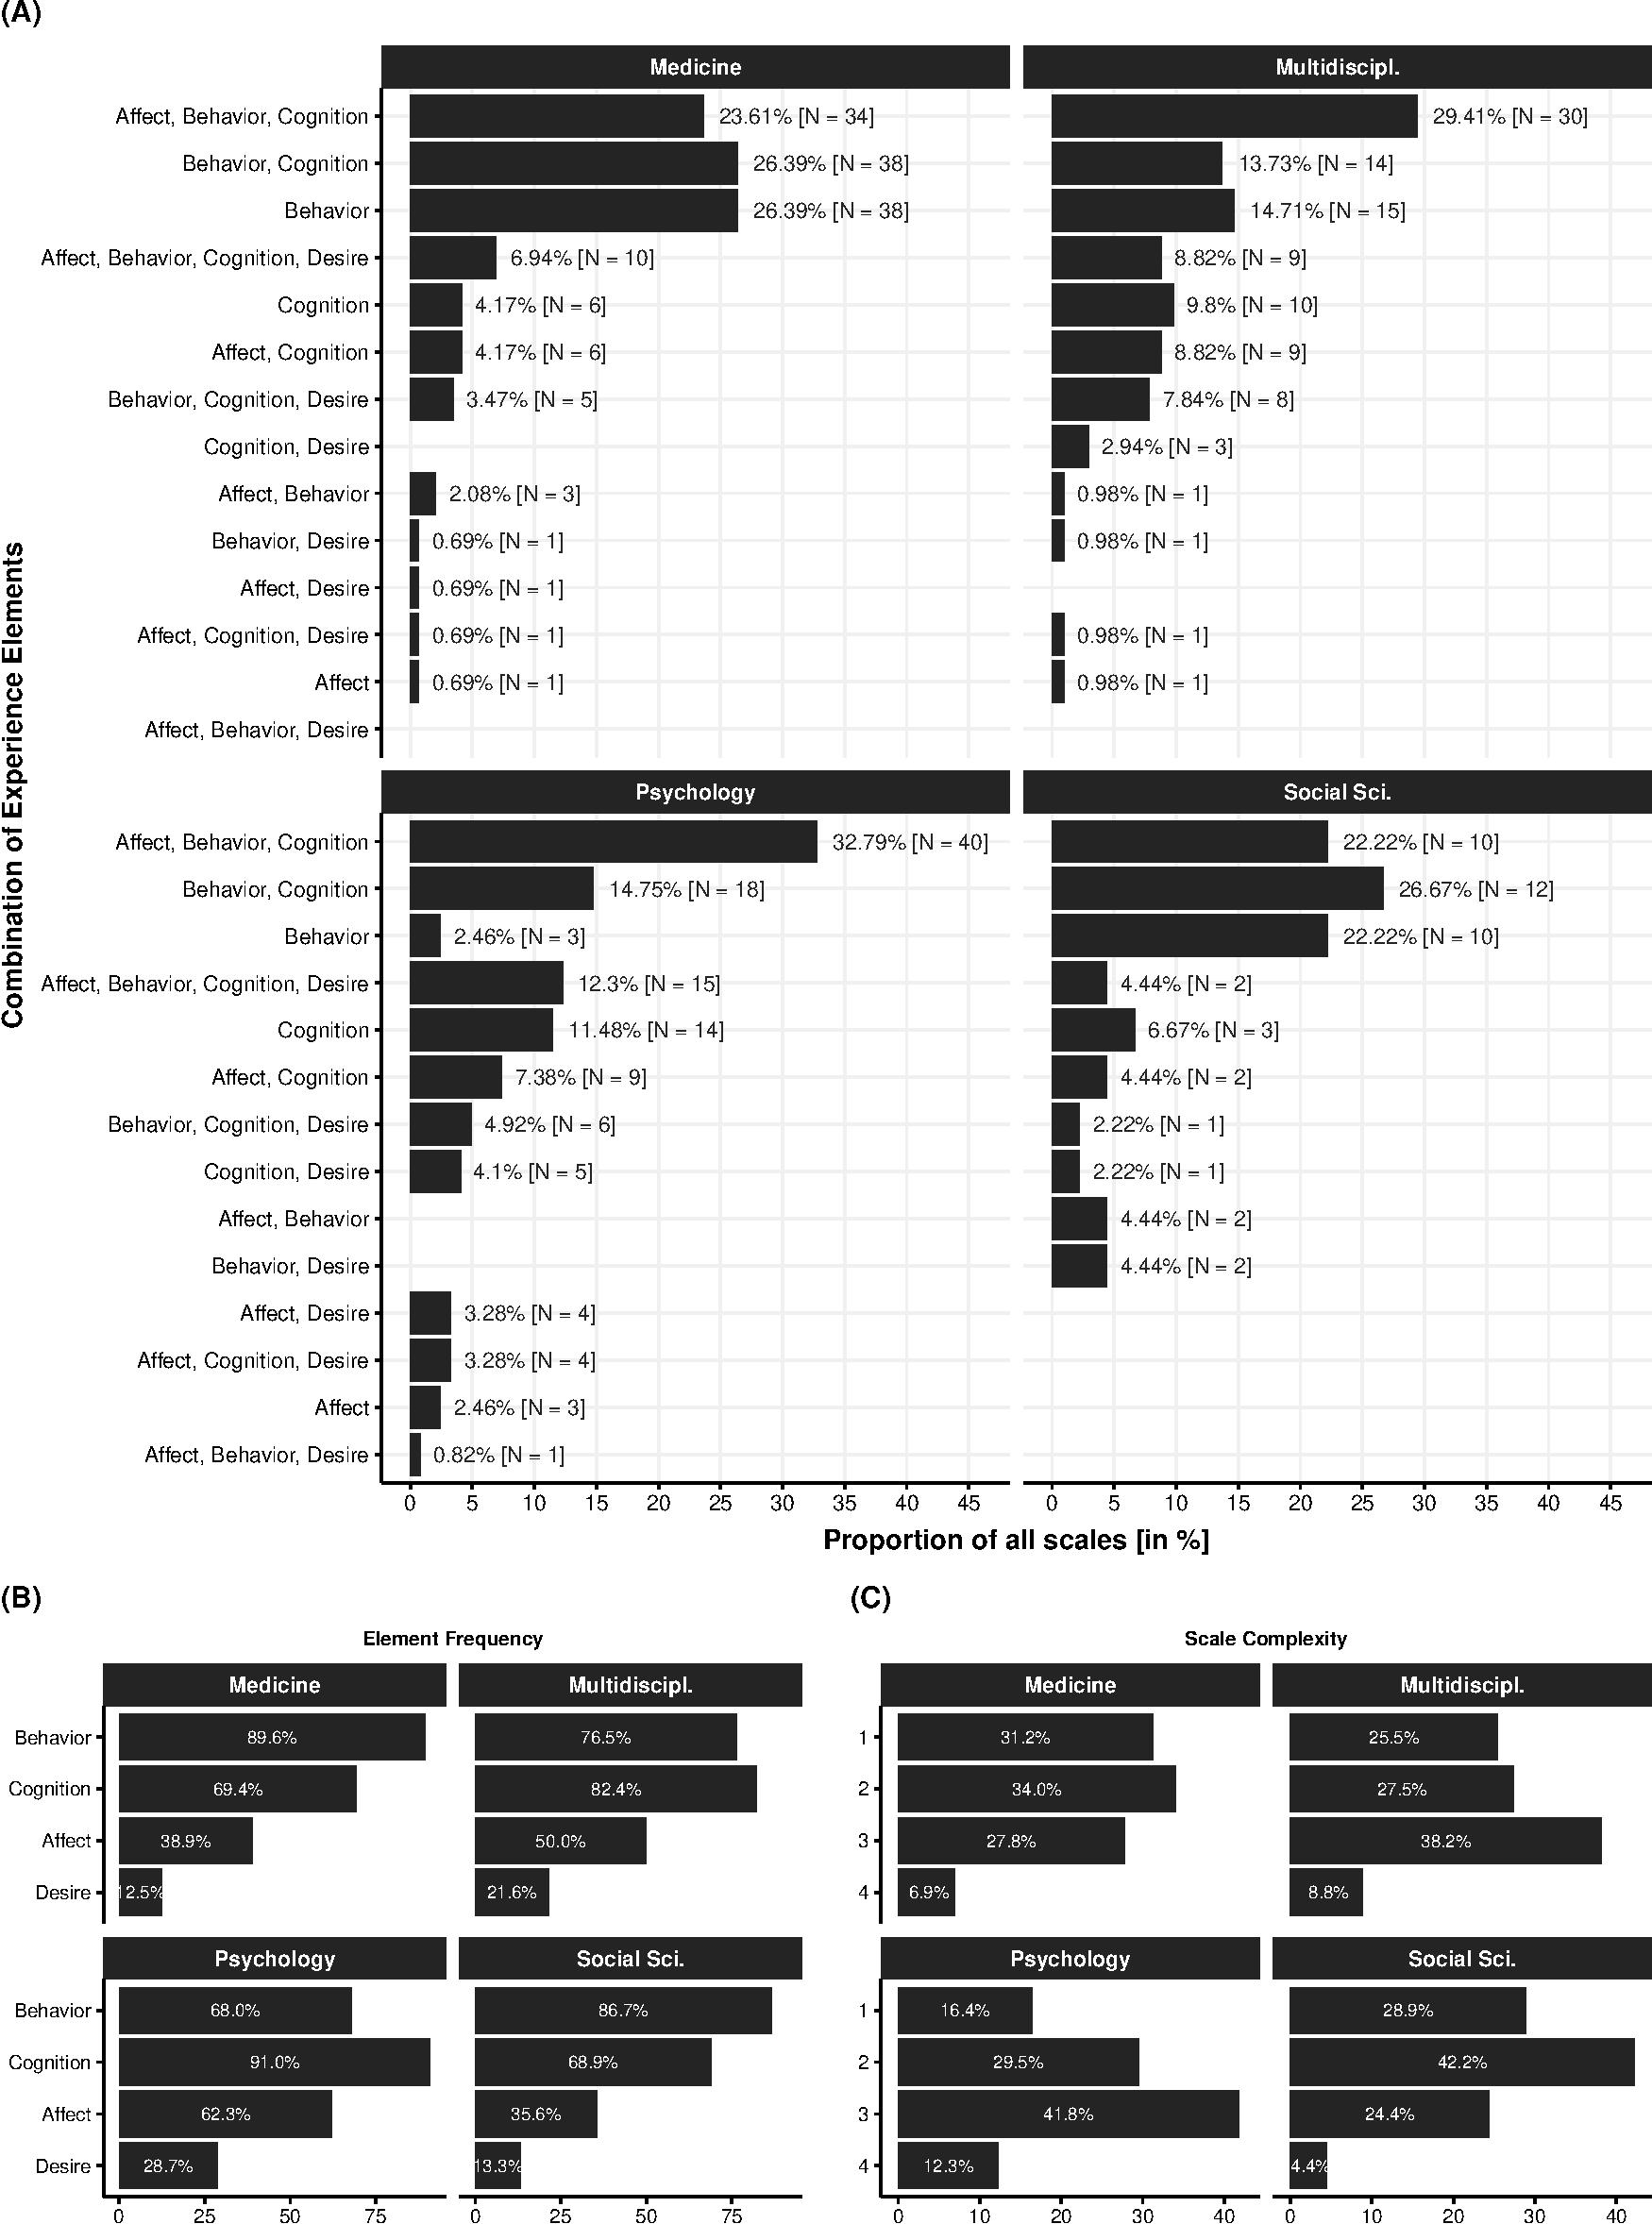
\includegraphics[width=\textwidth]{Figures/FieldPlotFreq-1}
\label{fig:FieldPlotFreq}
\end{figure}

\begin{figure}[h]
\centering
\caption{Average complexity (number of experience elements measured) for all scales that include a given experience aspect.}
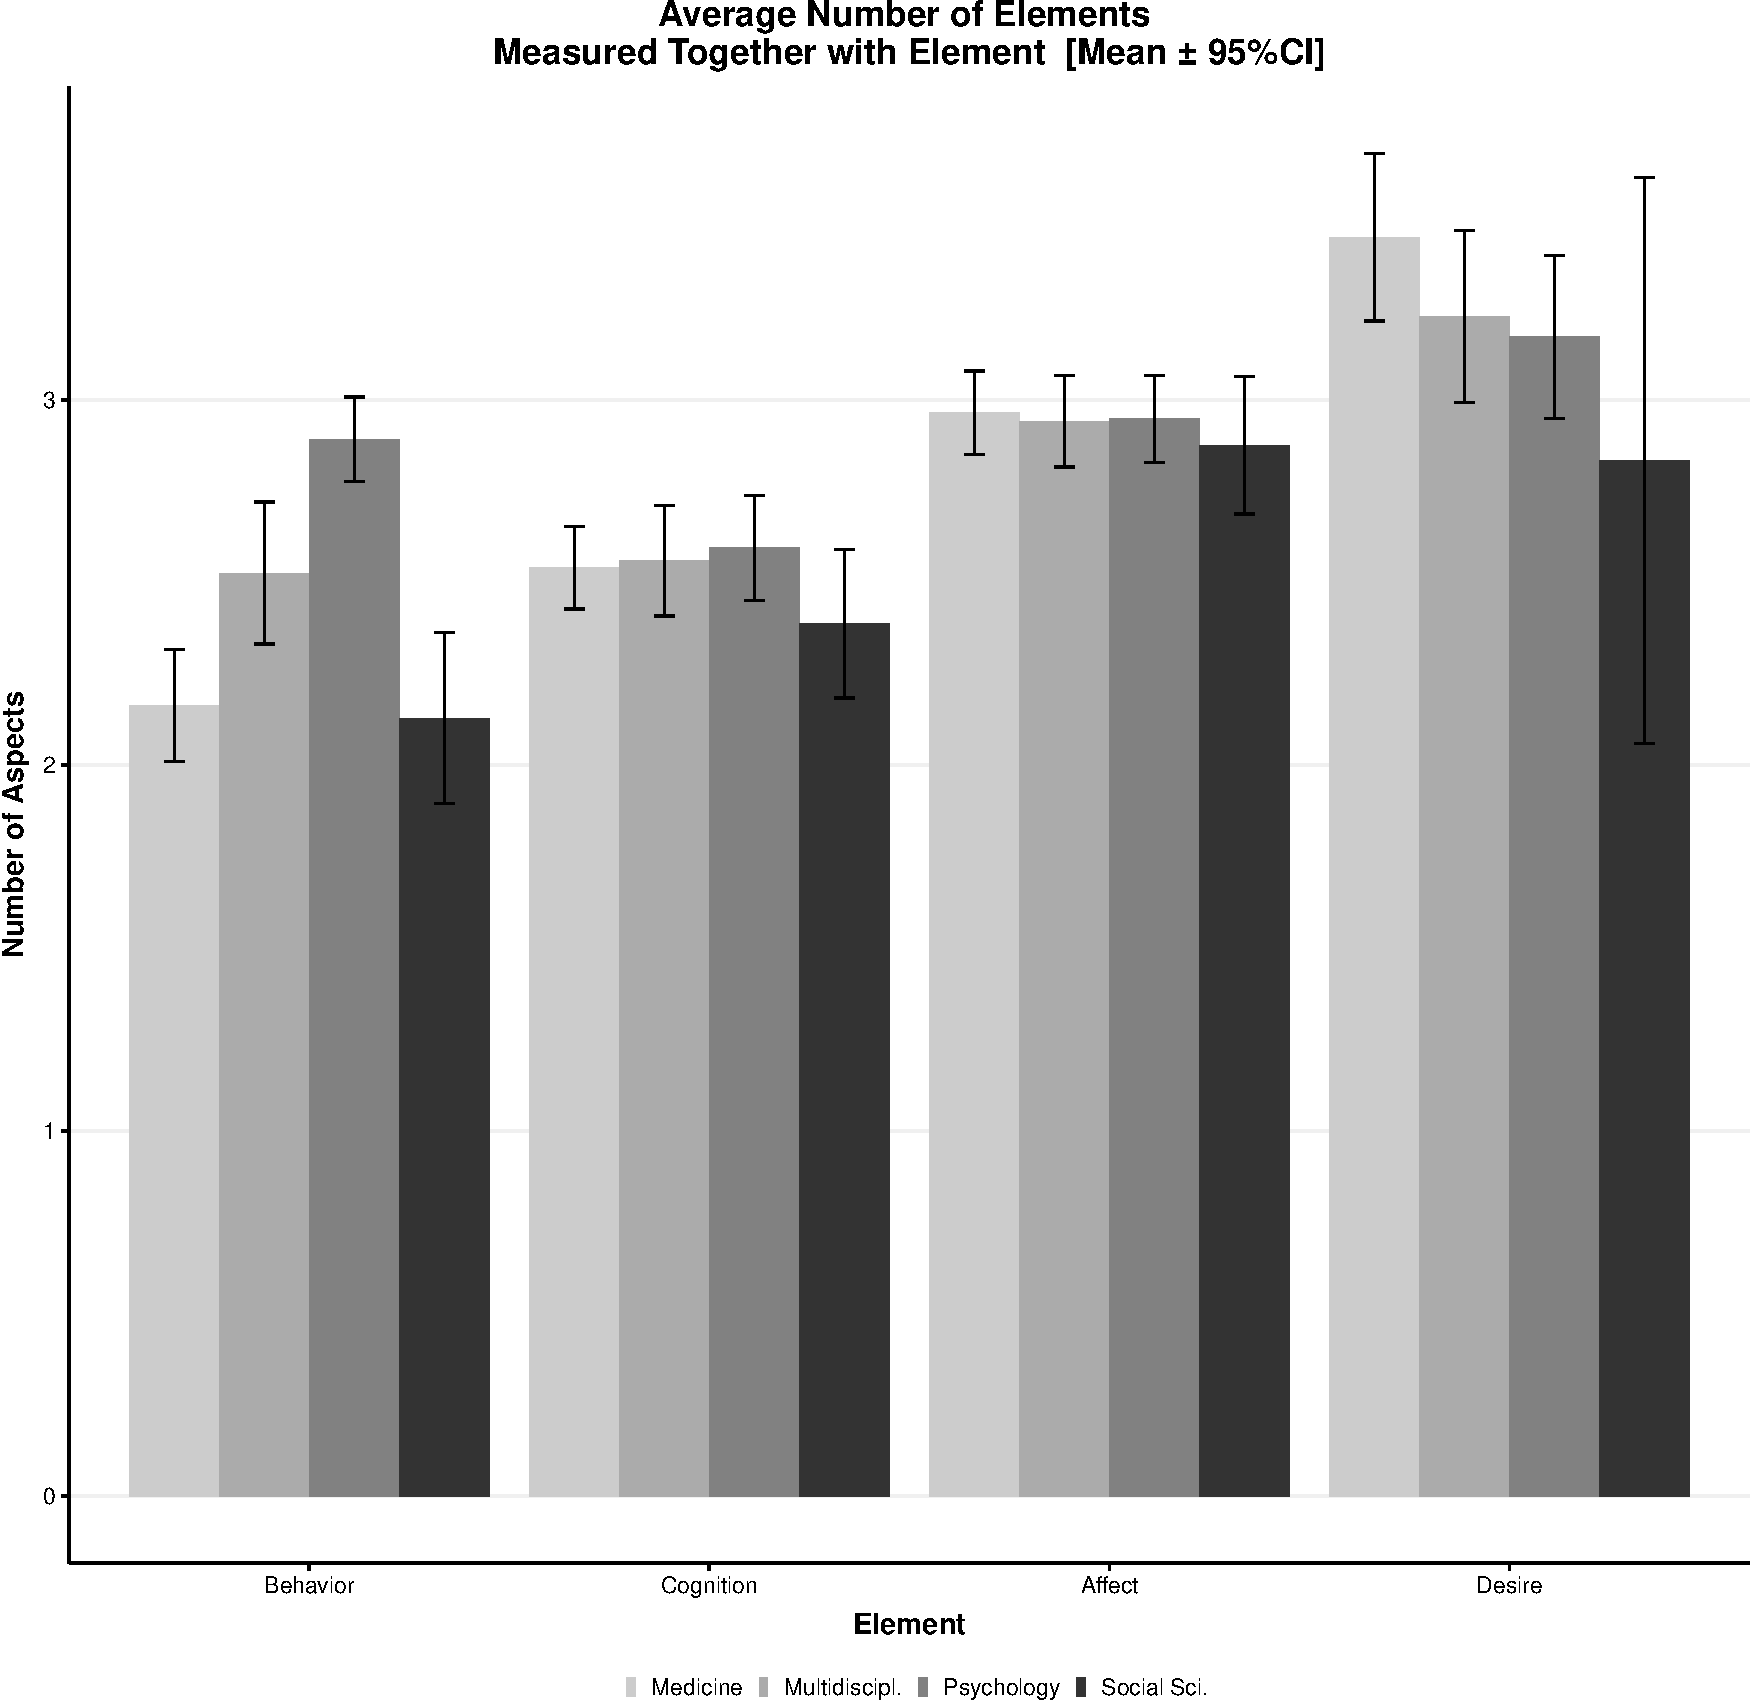
\includegraphics[width=\textwidth]{Figures/FieldElementComp-1}
\caption*{Note that these categories are not mutually exclusive (and thus not independent) because scales can include multiple experience aspects (i.e., higher complexity).}
\label{fig:FieldElementComp}
\end{figure}

\subsection{Theoretical Literature}

We then ran an additional literature search for theories of
acculturation\ldots{}

\subsubsection{Methods}

Methods here \ldots{}

\subsubsection{Results}

Results here \ldots{}\\
see Figure \ref{fig:ElementsTheories} and Table
\ref{tab:TheoriesElementCooccurrences}

\begin{figure}[h]
\centering
\caption{Scales: Bar graph of the experience element combinations.}
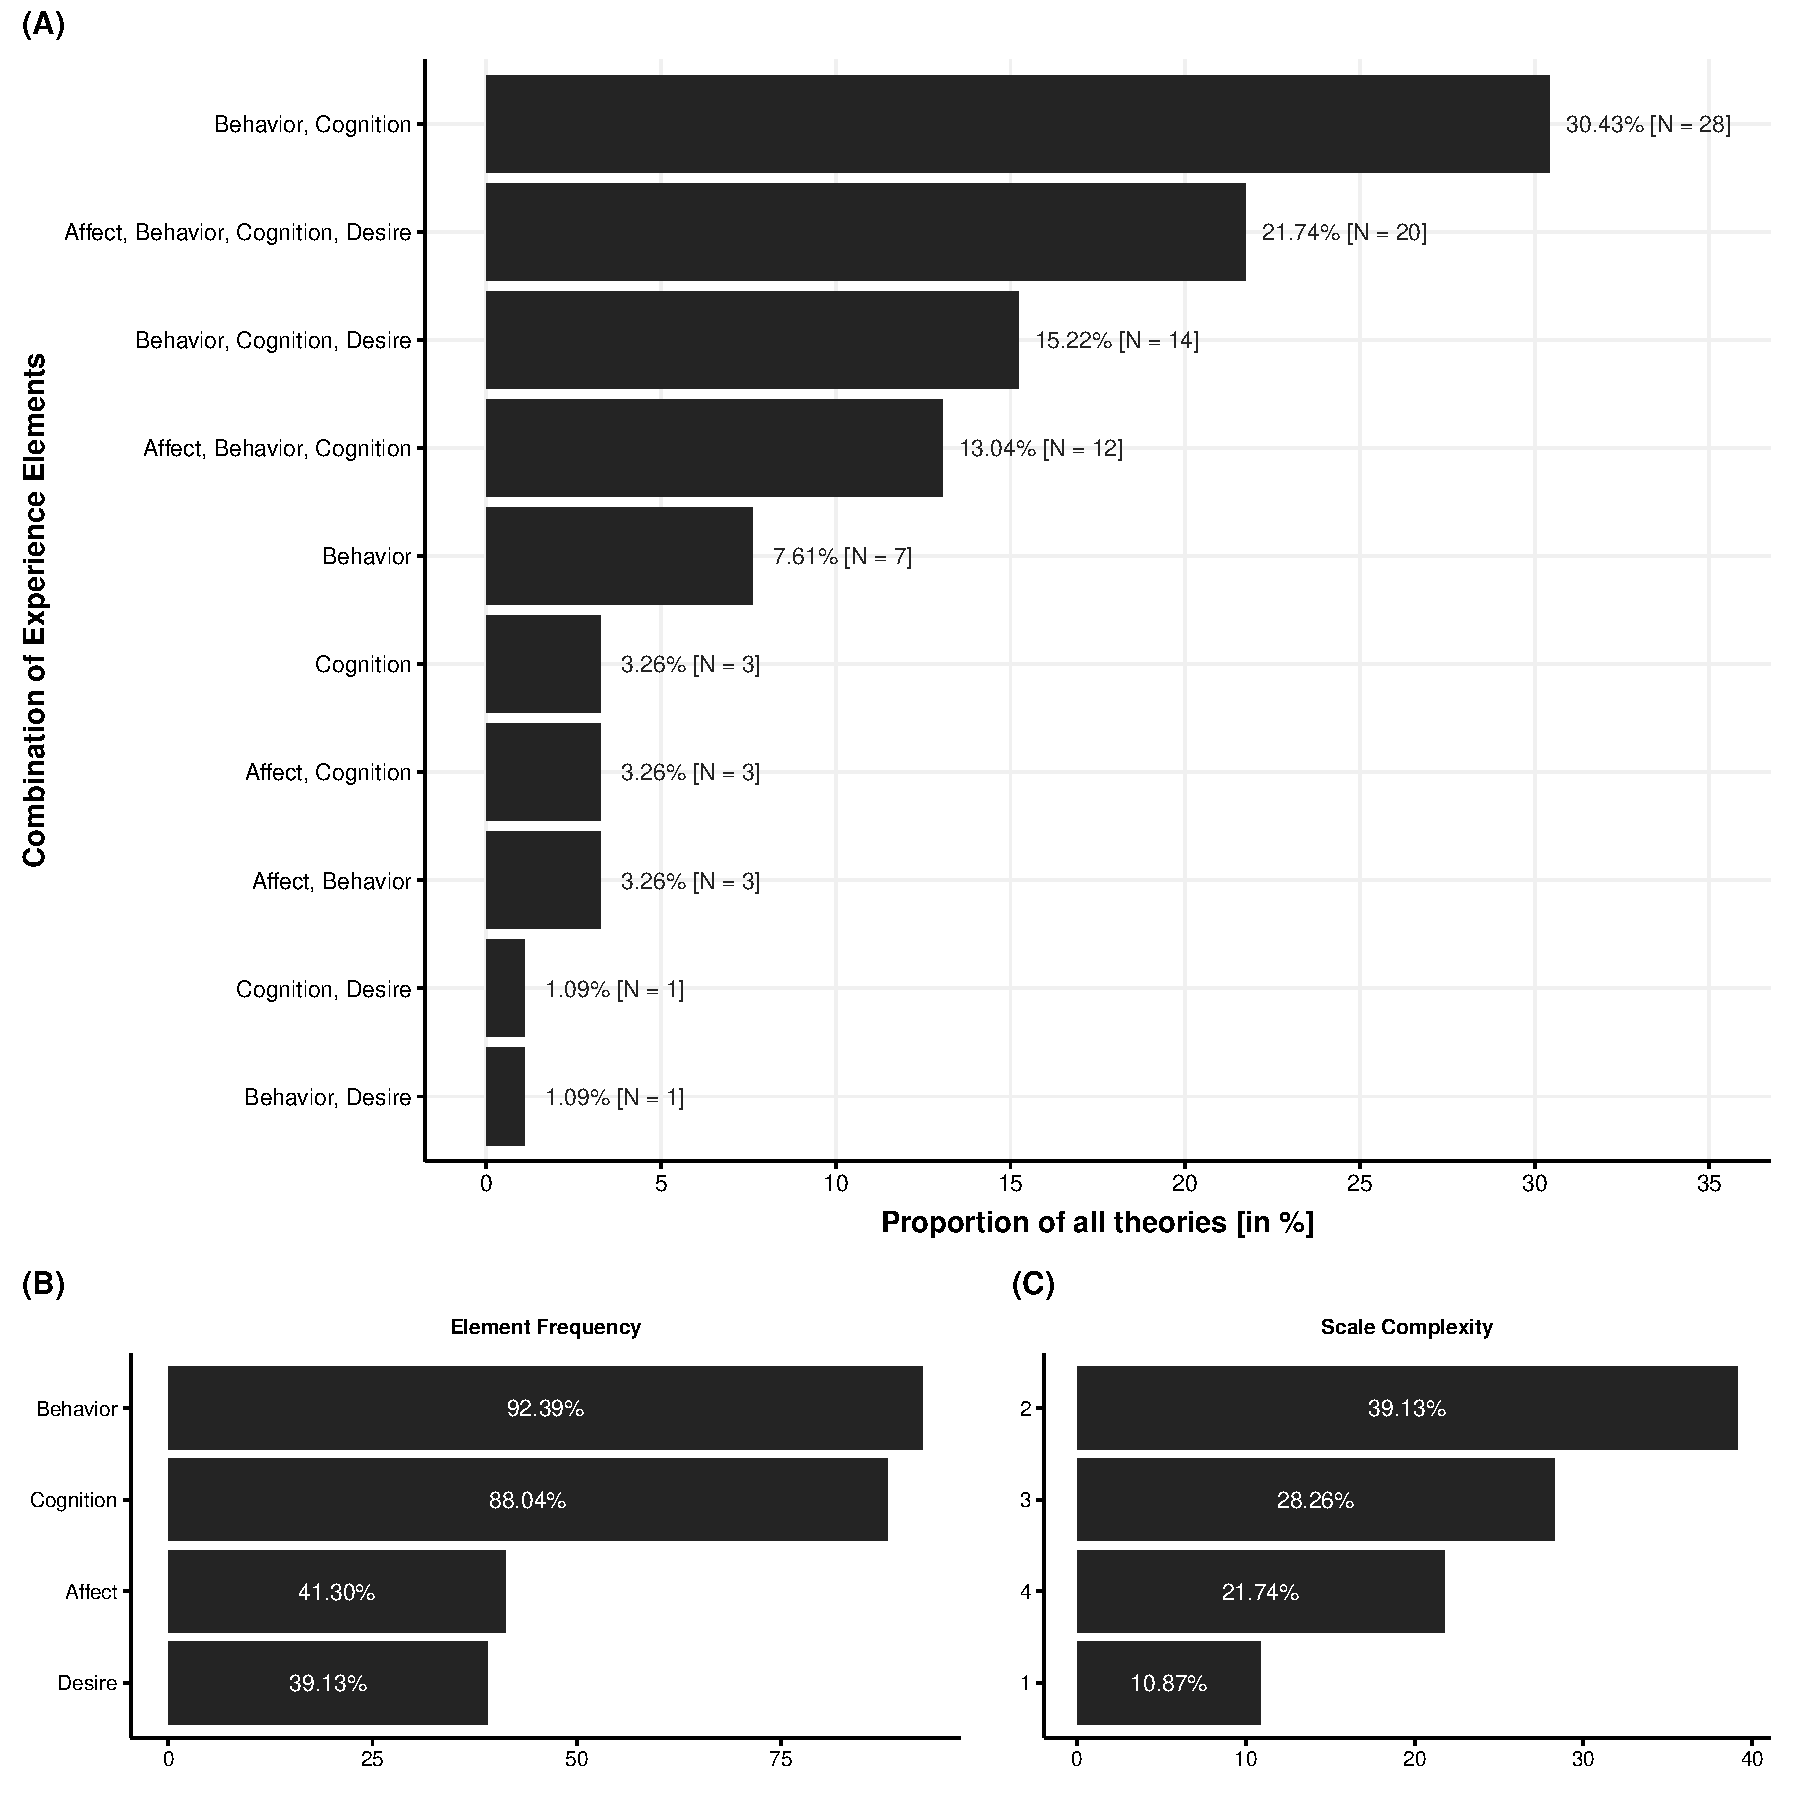
\includegraphics[width=\textwidth]{Figures/TheoriesFreq-1}
\label{fig:ElementsTheories}
\end{figure}

\begin{table}
\begin{minipage}[t][\textheight][t]{\textwidth}

\caption{\label{tab:TheoriesElementCooccurrences}Theoretical Literature: Element Co-occurrence Matrix}
\begin{tabular}[t]{lcccc}
\toprule
  & Affect & Behavior & Cognition & Desire\\
\midrule
Affect & 43 & 40 & 40 & 21\\
Behavior & 40 & 87 & 78 & 37\\
Cognition & 40 & 78 & 83 & 37\\
Desire & 21 & 37 & 37 & 38\\
\bottomrule
\end{tabular}
\end{minipage}
\end{table}

